\chapter{Resultados y discusión}

A continuación, se exponen y analizan los resultados alcanzados tras la realización del proyecto. La inclusión de archivos de log nos ofrece datos del estado del sistema que permiten estudiar la respuesta del brazo robótico ante los comandos.

\section{Resultados}

En términos generales, se han obtenido unos resultados satisfactorios en cuanto al funcionamiento del proyecto en todas sus etapas. 

A continuación se detallan los resultados obtenidos a partir de los datos recogidos de archivos de log y pruebas en vídeo. En el Anexo \ref{anexo:test} se recopila documentación en relación a las pruebas realizadas

\subsection{Test de eficiencia en recepción}

Se analiza el log de recepción de información para comprobar la correcta recepción de los datos.

En la figura \ref{fig:trec} se encuentran cuatro test en los que se representa la posición del hombro en función del tiempo relativo de test. Los frames incorrectamente recibidos se detectan cuando se recibe un 0 como posición articular.

\begin{figure}[tb]
  \centering
  \begin{minipage}[H]{1.1\textwidth}
    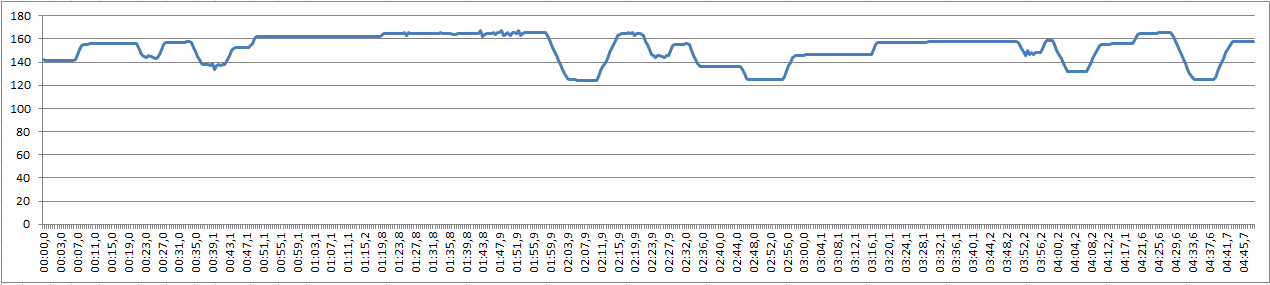
\includegraphics[width=\textwidth]{figuras/trec1.png}
  \end{minipage}
  \begin{minipage}[H]{1.1\textwidth}
    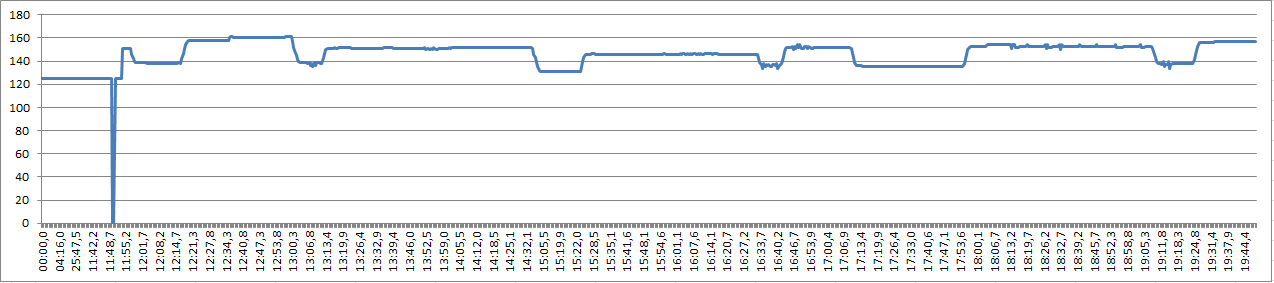
\includegraphics[width=\textwidth]{figuras/trec2.png}
  \end{minipage}
  \begin{minipage}[H]{1.1\textwidth}
    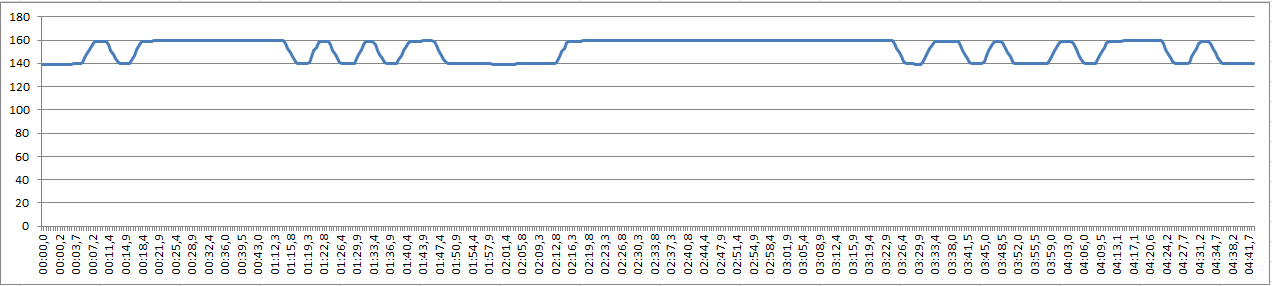
\includegraphics[width=\textwidth]{figuras/trec3.png}
  \end{minipage}
  \begin{minipage}[H]{1.1\textwidth}
    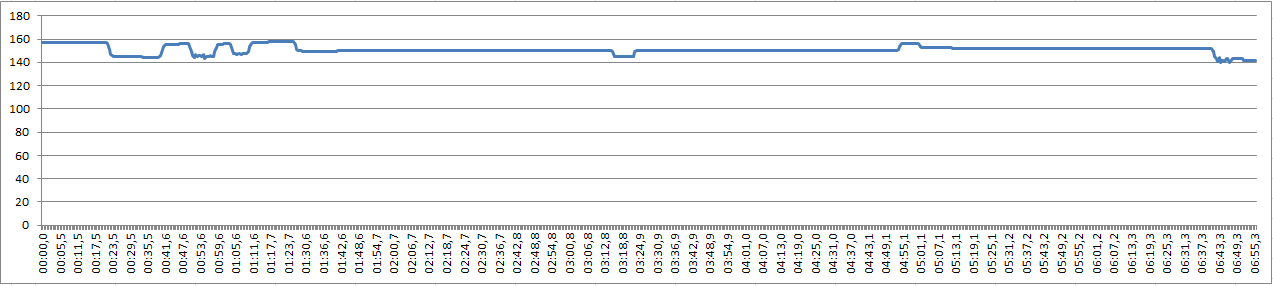
\includegraphics[width=\textwidth]{figuras/trec4.png}
  \end{minipage}
  \caption{Test de recepción de datos}\label{fig:trec}
\end{figure}

Analizando los datos de los logs, se puede observar que de un total de \textit{2864 frames} recibidos, tan sólo 2 lo hicieron de manera incorrecta. Teniendo en cuenta que RoboHealth Arm está programado para emitir un frame de estado cada 0,5 segundos, cabría esperar que enviara un total de 2984 frames. Esto supone una recepción adecuada del \textit{95,91\%} de los frames. Del porcentaje restante, el \textit{4,02\%} corresponden a mensajes teóricamente enviados por RHA pero que no han sido captados por el módulo XBee y el \textit{0.07\%} son mensajes recibidos que contienen información errónea.

\subsection{Test de eficiencia en emisión AT}\label{subsec:temat}

Se analiza una serie de envíos de información en modo AT y se compara con el movimiento del brazo para obtener el porcentaje de éxito en la emisión.

\begin{figure}[tb]
\centering
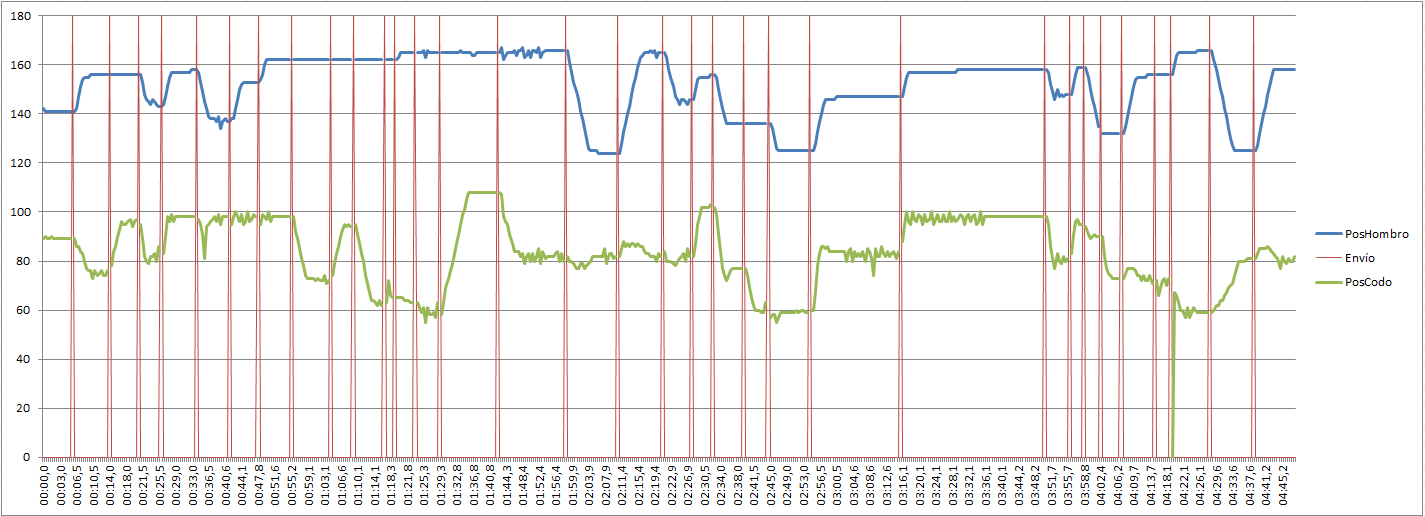
\includegraphics[width=1.1\textwidth]{figuras/temat.png}
\caption{Test de emisión AT de datos}
\label{fig:temat}
\end{figure}

En la figura \ref{fig:temat} se puede observar la posición de cada articulación con respecto al tiempo. Las líneas rojas verticales corresponden a envíos de información. Analizando la información, podemos concluir que, de \textit{33 envíos}, se recibieron correctamente 31. Dos envíos no llegaron a su destino, obteniendo un porcentaje de éxito del \textit{93,93\%}.

\subsection{Test de eficiencia en emisión API}


\subsection{Test de tiempos de respuesta}

El objetivo es usar los logs para obtener el valor del tiempo transcurrido entre que se envía un paquete de información y el robot empieza a moverse\footnote{En la práctica, será el valor del tiempo de recepción del frame de estado en el que se detecta un cambio de posición en las articulaciones, por lo que cabe esperar que el tiempo de respuesta sea algo menor}. En la figura \ref{fig:tresp} se puede ver el detalle de una de estas respuestas.

\begin{figure}[tb]
\centering
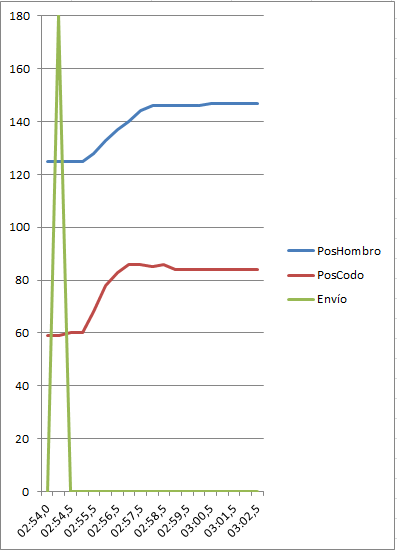
\includegraphics[width=0.4\textwidth]{figuras/tresp.png}
\caption{Detalle de la respuesta}
\label{fig:tresp}
\end{figure}

El tiempo de respuesta medio resultante es de \textit{0.73 segundos}. Este valor se obtiene como la media del tiempo de respuesta de una muestra con \textit{31 envíos exitosos} de información aunque hay que tener en cuenta que el periodo de refresco de la información de las articulaciones que proporciona el RHA es de aproximadamente 0.5 segundos. Se puede comprobar la varianza de los datos que demuestra esta situación en los datos adjuntos en el Anexo \ref{anexo:test} (tabla \ref{tab:treac}). Una varianza representativa\footnote{La varianza es representativa en un caso como este cuando el error medio se aproxima al valor medio de las muestras} dificulta medir con precisión el tiempo de respuesta en una muestra con datos limitados, como es el caso.

\subsection{Test de MQTT}

A través de pruebas en vídeo sincronizadas con los archivos de log de envío, se trata de obtener un porcentaje de éxito de los comandos desde MQTT.

\begin{figure}[tb]
  \centering
  \begin{minipage}[H]{1\textwidth}
    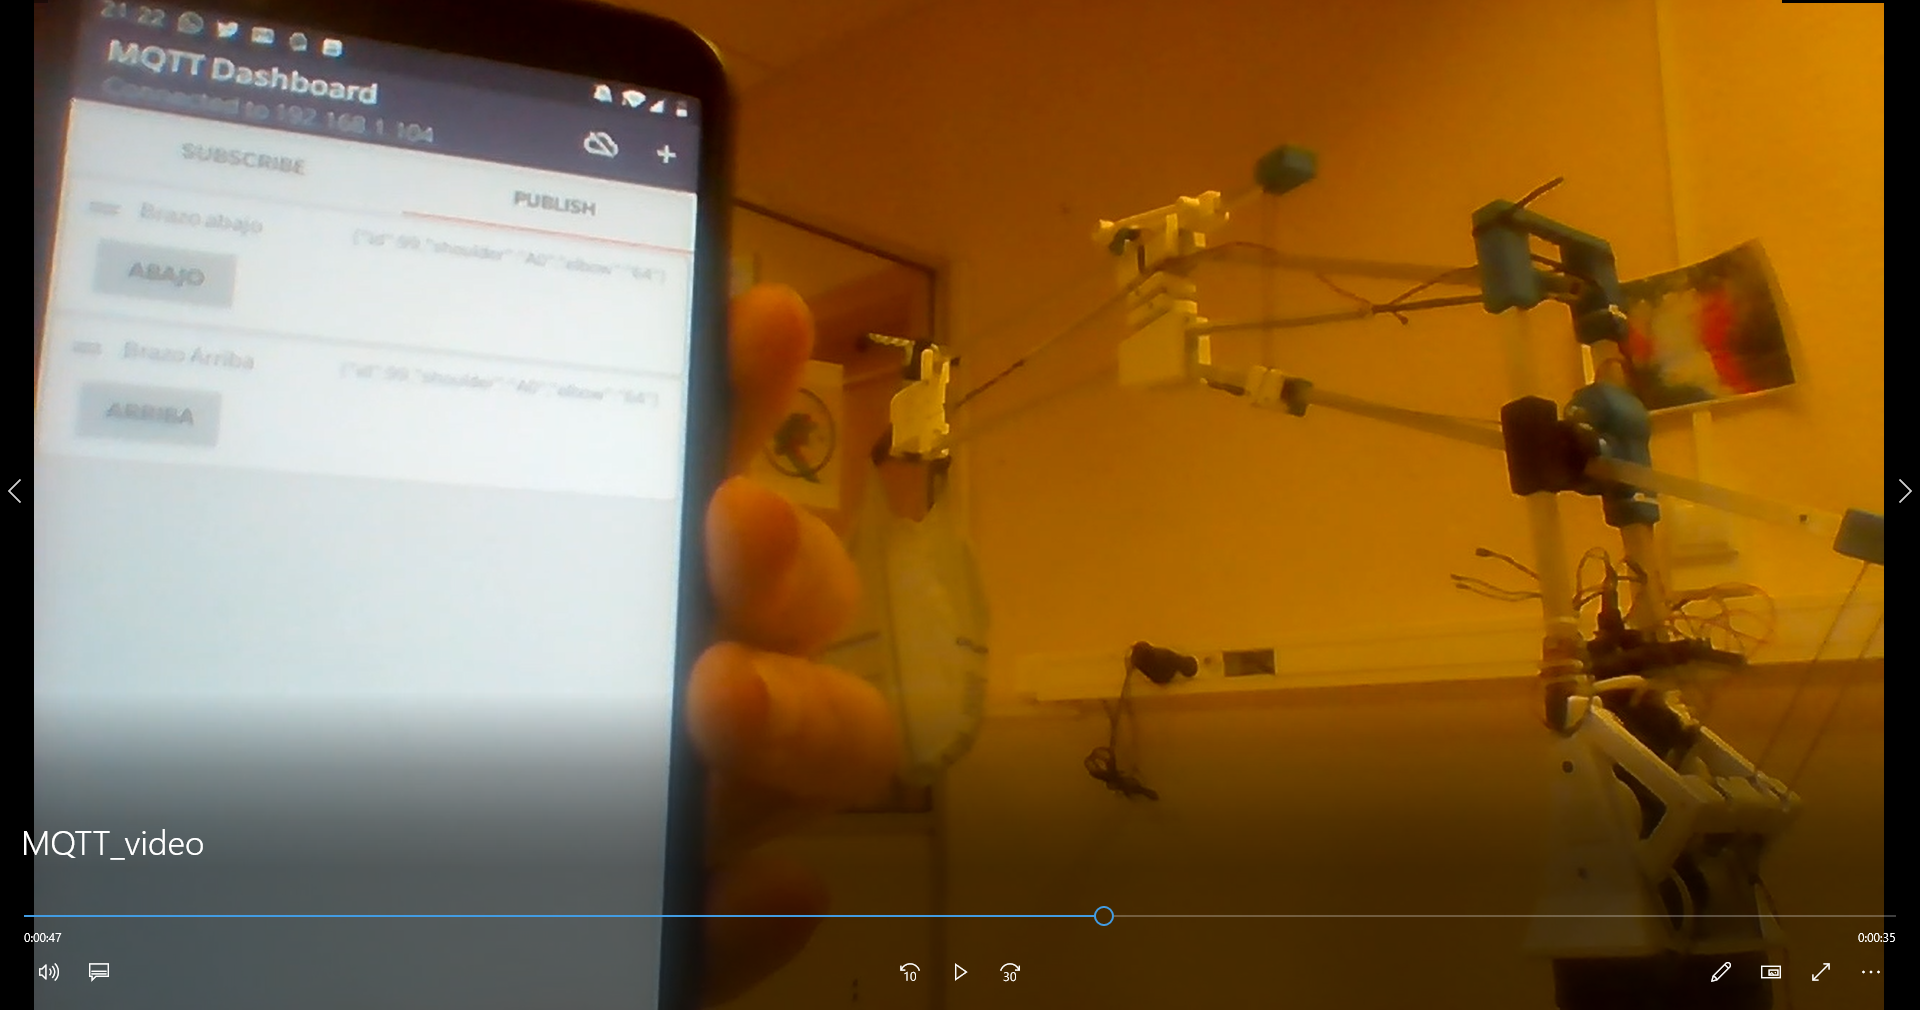
\includegraphics[width=\textwidth]{figuras/MQTTVideo.png}
  \end{minipage}
  \begin{minipage}[H]{1.1\textwidth}
    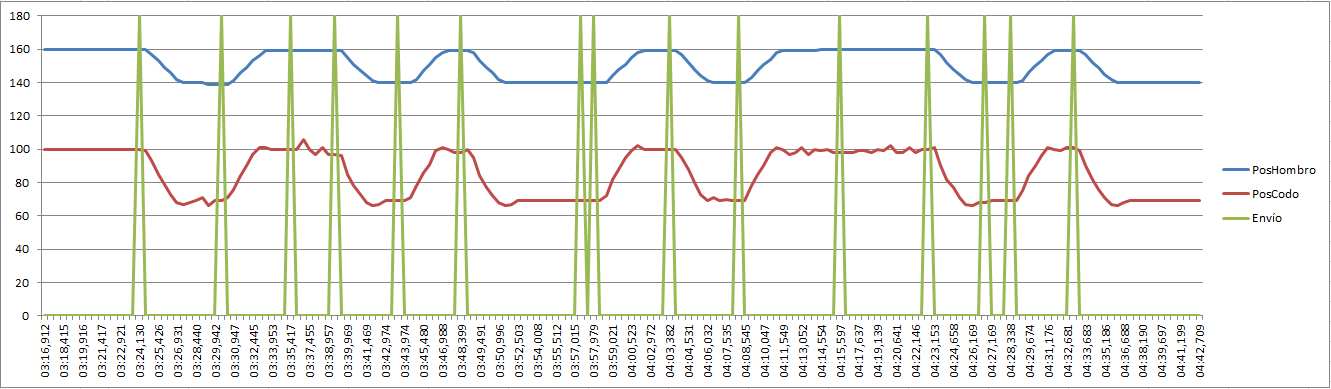
\includegraphics[width=\textwidth]{figuras/tmqtt.png}
  \end{minipage}
  \caption{Test de uso vía MQTT}\label{fig:tmqtt}
\end{figure}

Con la figura \ref{fig:tmqtt} uno puede hacerse una idea del proceso seguido. Se aisló un log de tal manera que sus datos coincidieran con la grabación de las acciones realizadas desde un dispositivo conectado a la red MQTT y la respuesta del brazo. Así, contando las acciones indicadas desde MQTT, el número de envíos de información vía XBee y las reacciones del brazo; se puede sacar el rendimiento de la red en cada punto.

Los resultados son los siguientes: 17 veces se mandó al brazo cambiar su posición desde el móvil. De ellas, 15 fueron transmitidas a través de XBee y se provocaron 11 movimientos del brazo.

En porcentajes, el brazo ejecutó el 65\% de las órdenes enviadas desde el móvil, siendo el 88\% de ellas las que se transmitieron vía radiofrecuencia.

\section{Discusión}

Como se ha comentado antes, se han obtenido buenos resultados en general. Se presenta un a forma versátil y fiable de comandar el robot.

En cuanto a la recepción, los resultados son excepcionales. Un porcentaje muy alto (95,91\%) de los frames de estado son captados por la red domótica. Estos frames de estado, en el funcionamiento usual de la red, cumplirían la única función de representar en la interfaz la posición articular del hombro y del codo con la tasa de refresco programada en RHA. La pérdida de un frame de estado no es crítica en sí porque la representación mantendría la posición previa hasta recibir un nuevo frame de estado medio segundo después. Lo crítico es evitar la recepción por parte de la red domótica de un frame de estado, identificado como tal, pero con información corrupta, a medias o inexistente. En ese caso, el frame pasaría los filtros de representación y acabaría mostrando una posición errónea. Los datos demuestran que esta situación es residual (0.07\%) así que no supone mayor problema.

La emisión de órdenes en modo AT mantiene un porcentaje de éxito bastante alto (93,93\%) haciendo uso de su sencillez y de ser el modo principal sobre el que está pensado el protocolo de comunicación y, por lo tanto, estar más probado.

En el envío en modo API aumenta la tasa de error a pesar de mantener un porcentaje de éxito bastante sólido. Probablemente sea debido a un frame más largo que requiere de más comprobaciones antes de ser interpretado y a un código de recepción imperfecto. En parte, es el precio a pagar por las ventajas que aporta (explicado en detalle en el apartado \ref{subsubsec:modoscom}).

Los tiempos de respuesta a los envíos de comandos son realmente buenos. A pesar de la dificultad para medirlos de manera precisa, se puede asegurar que no suben del segundo; lo que es más que suficiente para la aplicación descrita.

MQTT introduce una etapa más de transmisión de la información en la que se puede perder. En este caso, las pruebas muestran que los escasos comandos MQTT perdidos se han producido en situaciones en las que se enviaban de manera extremadamente consecutiva. Esto hace que su pérdida no resulte un verdadero problema. Sin embargo, en este test sí que ha aumentado el porcentaje de error en la transmisión de Node-RED al brazo. Hay pocas explicaciones ya que se trata de exactamente el mismo script usado en la sección \ref{fig:temat}, pero podría deberse al tamaño excesivamente limitado de la muestra grabada en vídeo.

Por último, merece la pena indicar que, aunque no existan pruebas ni datos que lo demuestre, los errores de emisión parece que tienden a producirse cuando el brazo robótico entra en un estado de oscilación. Esta situación es relativamente frecuente y puede observarse en las gráficas previas, como es el caso de la figura \ref{fig:tmqtt}.